% ============================================================
%  Section 3 — TabgenQA System Overview
%  For: TabgenQA: a Platform to Generate and Evaluate
%       Non-Relational Multi-Table Numerical QA Benchmarks
%  CIKM 2025 Demo Track
% ============================================================

\section{System Overview}
\label{sec:system}

TabgenQA is organized as a three-tier web application
(Figure~\ref{fig:architecture}) comprising a React-based single-page
frontend, a FastAPI backend, and the Gradino generation
library~\cite{gradino} together with third-party large language model
(LLM) APIs.
A lightweight task manager on the backend tracks the lifecycle of every
generation and evaluation job, persisting results to disk so that history
and leaderboard data survive service restarts.
All long-running operations stream real-time progress to the browser via
Server-Sent Events (SSE), giving users immediate feedback without page
reloads.
The complete platform is distributed as a Docker Compose application;
an optional GPU service can be enabled to serve open-weight models
through a vLLM~\cite{kwon2023vllm} endpoint.

\begin{figure}[t]
  \centering
  %% --------------------------------------------------------
  %% FIGURE TO DRAW: three-column architecture diagram.
  %%
  %% Left column — "Frontend (React / Tailwind CSS)":
  %%   Three stacked rounded boxes labelled
  %%   "Generate Tab", "History Tab", "Leaderboard Tab".
  %%
  %% Middle column — "Backend (FastAPI)":
  %%   Four stacked rounded boxes labelled
  %%   "REST API", "Task Manager", "SSE Progress Stream",
  %%   "Eval Runner (subprocess)".
  %%
  %% Right column — "External Services":
  %%   Two rounded boxes:
  %%     (top)    "Gradino Library"   [grey/hatched to signal black-box]
  %%     (bottom) "LLM APIs"
  %%              (sub-labels: OpenAI · Anthropic Claude ·
  %%               Google Gemini · vLLM / HuggingFace)
  %%
  %% Arrows:
  %%   Frontend ↔ Backend : bidirectional, labelled "HTTP / SSE"
  %%   Backend  → Gradino : right arrow, labelled "subprocess"
  %%   Backend  → LLM APIs: right arrow, labelled "HTTPS"
  %% --------------------------------------------------------
  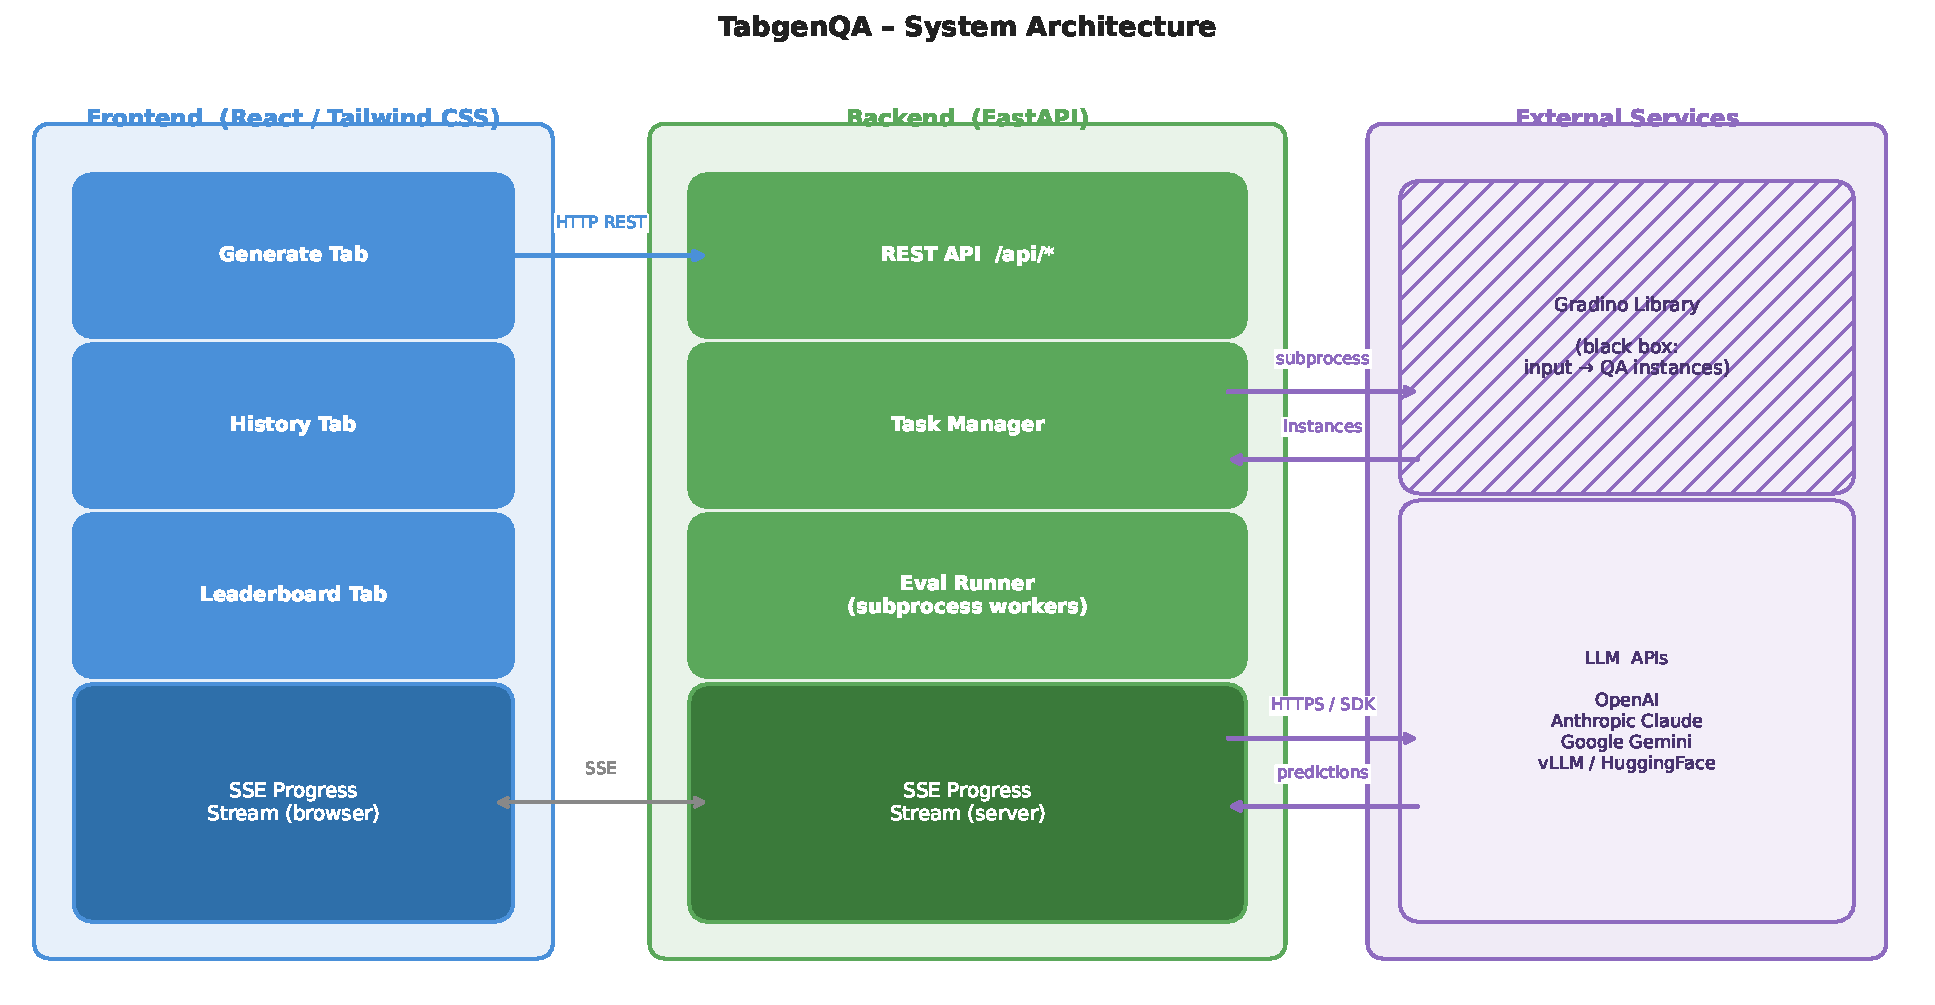
\includegraphics[width=\linewidth]{figures/architecture}
  \caption{High-level architecture of TabgenQA. The React frontend
    communicates with the FastAPI backend via REST and SSE; the backend
    delegates benchmark generation to Gradino and model inference to
    third-party LLM provider APIs.}
  \label{fig:architecture}
\end{figure}

\smallskip\noindent\textbf{Benchmark Generation.}
The \emph{Generate} tab exposes a parameter form through which the user
configures the benchmark to produce (Figure~\ref{fig:ui}a).
The configurable parameters are:
(i)~\emph{domain}, chosen from
  \texttt{environmental}, \texttt{finance},
  \texttt{healthcare}, and \texttt{products};
(ii)~\emph{question type} (\texttt{sum}, \texttt{average}, or
  \texttt{superlative});
(iii)~\emph{number of tables} to join
  ($2$–$20$, or \texttt{auto} for a full ablation sweep over
  $\{2,3,5,10,20\}$);
(iv)~\emph{number of samples} per configuration; and
(v)~advanced options for column cardinality, number of columns, and
  whether multi-hop reasoning should follow a sequential chain across
  tables.
Upon submission the backend launches Gradino as a subprocess and forwards
its progress to the browser via SSE.
Gradino~\cite{gradino} is treated as a black box in TabgenQA: it receives
the parameters above and returns, for each
\emph{(num\_tables, question\_type, perturbation)} combination, a data
table whose rows encode the fields
\textsc{Question} (natural-language question),
\textsc{Table} (one or more HTML-serialised relational tables),
\textsc{Label} (gold numerical answer),
\textsc{SQL Query} (derivation trace),
\textsc{Method}, and \textsc{Constraints}.
TabgenQA flattens this output into a list of JSON instances—each
assigned a unique identifier—and offers the result as a downloadable
archive in both JSON and CSV formats.

\smallskip\noindent\textbf{Instance Review and Editing.}
The \emph{History} tab (Figure~\ref{fig:ui}b) lists all past generation
runs ordered by creation timestamp and filterable by domain, question
type, and number of tables.
Each entry in the list shows the configuration summary, the run status
(\emph{pending} / \emph{running} / \emph{done} / \emph{failed}), and the
number of instances produced.
From a history entry the user can download the raw instances or trigger
an evaluation run directly, enabling iterative benchmark curation—for
example, discarding a domain or perturbation type and regenerating—without
leaving the interface.

\smallskip\noindent\textbf{Evaluation Runner.}
Clicking \emph{Evaluate} on a history entry opens a configuration modal
(Figure~\ref{fig:ui}c) in which the user selects the LLM to be evaluated.
TabgenQA supports four provider families:
(i)~OpenAI-compatible models (e.g., \texttt{gpt-4o-mini});
(ii)~Anthropic Claude models via the Anthropic SDK;
(iii)~Google Gemini models via Google's OpenAI-compatible endpoint, which
  requires no additional SDK; and
(iv)~self-hosted open-weight models served through a
  vLLM~\cite{kwon2023vllm} instance, enabling evaluation without API
  costs or data-sharing concerns.
For each instance the model receives a chain-of-thought prompt that
includes the HTML table(s) and the question; the prompt instructs the
model to conclude with the token sequence ``\texttt{Final answer:}''
followed exclusively by the numerical result~\cite{wei2022chain}.
The predicted answer is extracted from the final-answer span, stripped of
Markdown formatting, and scored against the gold label using
exact numerical match (tolerance $\pm 0.005$) and token-level
F1~\cite{rajpurkar-etal-2016-squad}.
Inference progress is streamed to the browser in real time; upon
completion the backend persists the full prediction set—including the
model's chain-of-thought reasoning—alongside aggregate accuracy and
average F1 statistics.

\smallskip\noindent\textbf{Leaderboard and Analytics.}
The \emph{Leaderboard} tab (Figure~\ref{fig:ui}d) aggregates all
completed evaluation runs into a ranked table sorted by accuracy.
Each row displays the model name, provider type (colour-coded badge), the
evaluated benchmark run, accuracy, average F1, and the number of
instances scored.
Clicking a row opens a slide-in detail panel that lists every instance
with its gold answer, predicted answer, and toggles to expand the
supporting HTML table(s) and the full model reasoning trace.
Three filter tabs (\emph{All} / \emph{Correct} / \emph{Wrong}) allow the
practitioner to isolate failure modes and examine systematic errors across
question types, perturbation conditions, and numbers of tables.

\begin{figure}[t]
  \centering
  %% --------------------------------------------------------
  %% FIGURE TO DRAW: four-panel screenshot figure (2 × 2 grid).
  %%
  %% Panel (a) — Generate tab:
  %%   Show the parameter form (domain dropdown open or showing a
  %%   selected value, num-tables and num-samples controls) and the
  %%   SSE progress bar partially filled during an active run.
  %%   Label: "(a) Benchmark generation with live progress."
  %%
  %% Panel (b) — History tab:
  %%   Show two or three completed task cards with the filter-chip
  %%   bar at the top (Domain · Question Type · Num Tables) and
  %%   per-card Download and Evaluate buttons.
  %%   Label: "(b) Run history with filtering."
  %%
  %% Panel (c) — Evaluate modal:
  %%   Show the model-type selector (OpenAI selected), model-name
  %%   input, API key field (redacted), and the live progress bar
  %%   filling during inference.
  %%   Label: "(c) Model evaluation configuration."
  %%
  %% Panel (d) — Leaderboard + detail panel:
  %%   Left half: ranked leaderboard table (3–4 rows visible).
  %%   Right half: slide-in panel for one selected row, showing
  %%   one instance with gold answer, predicted answer (coloured
  %%   green/red), and the reasoning trace in a monospace block.
  %%   Label: "(d) Leaderboard with per-instance detail."
  %% --------------------------------------------------------
  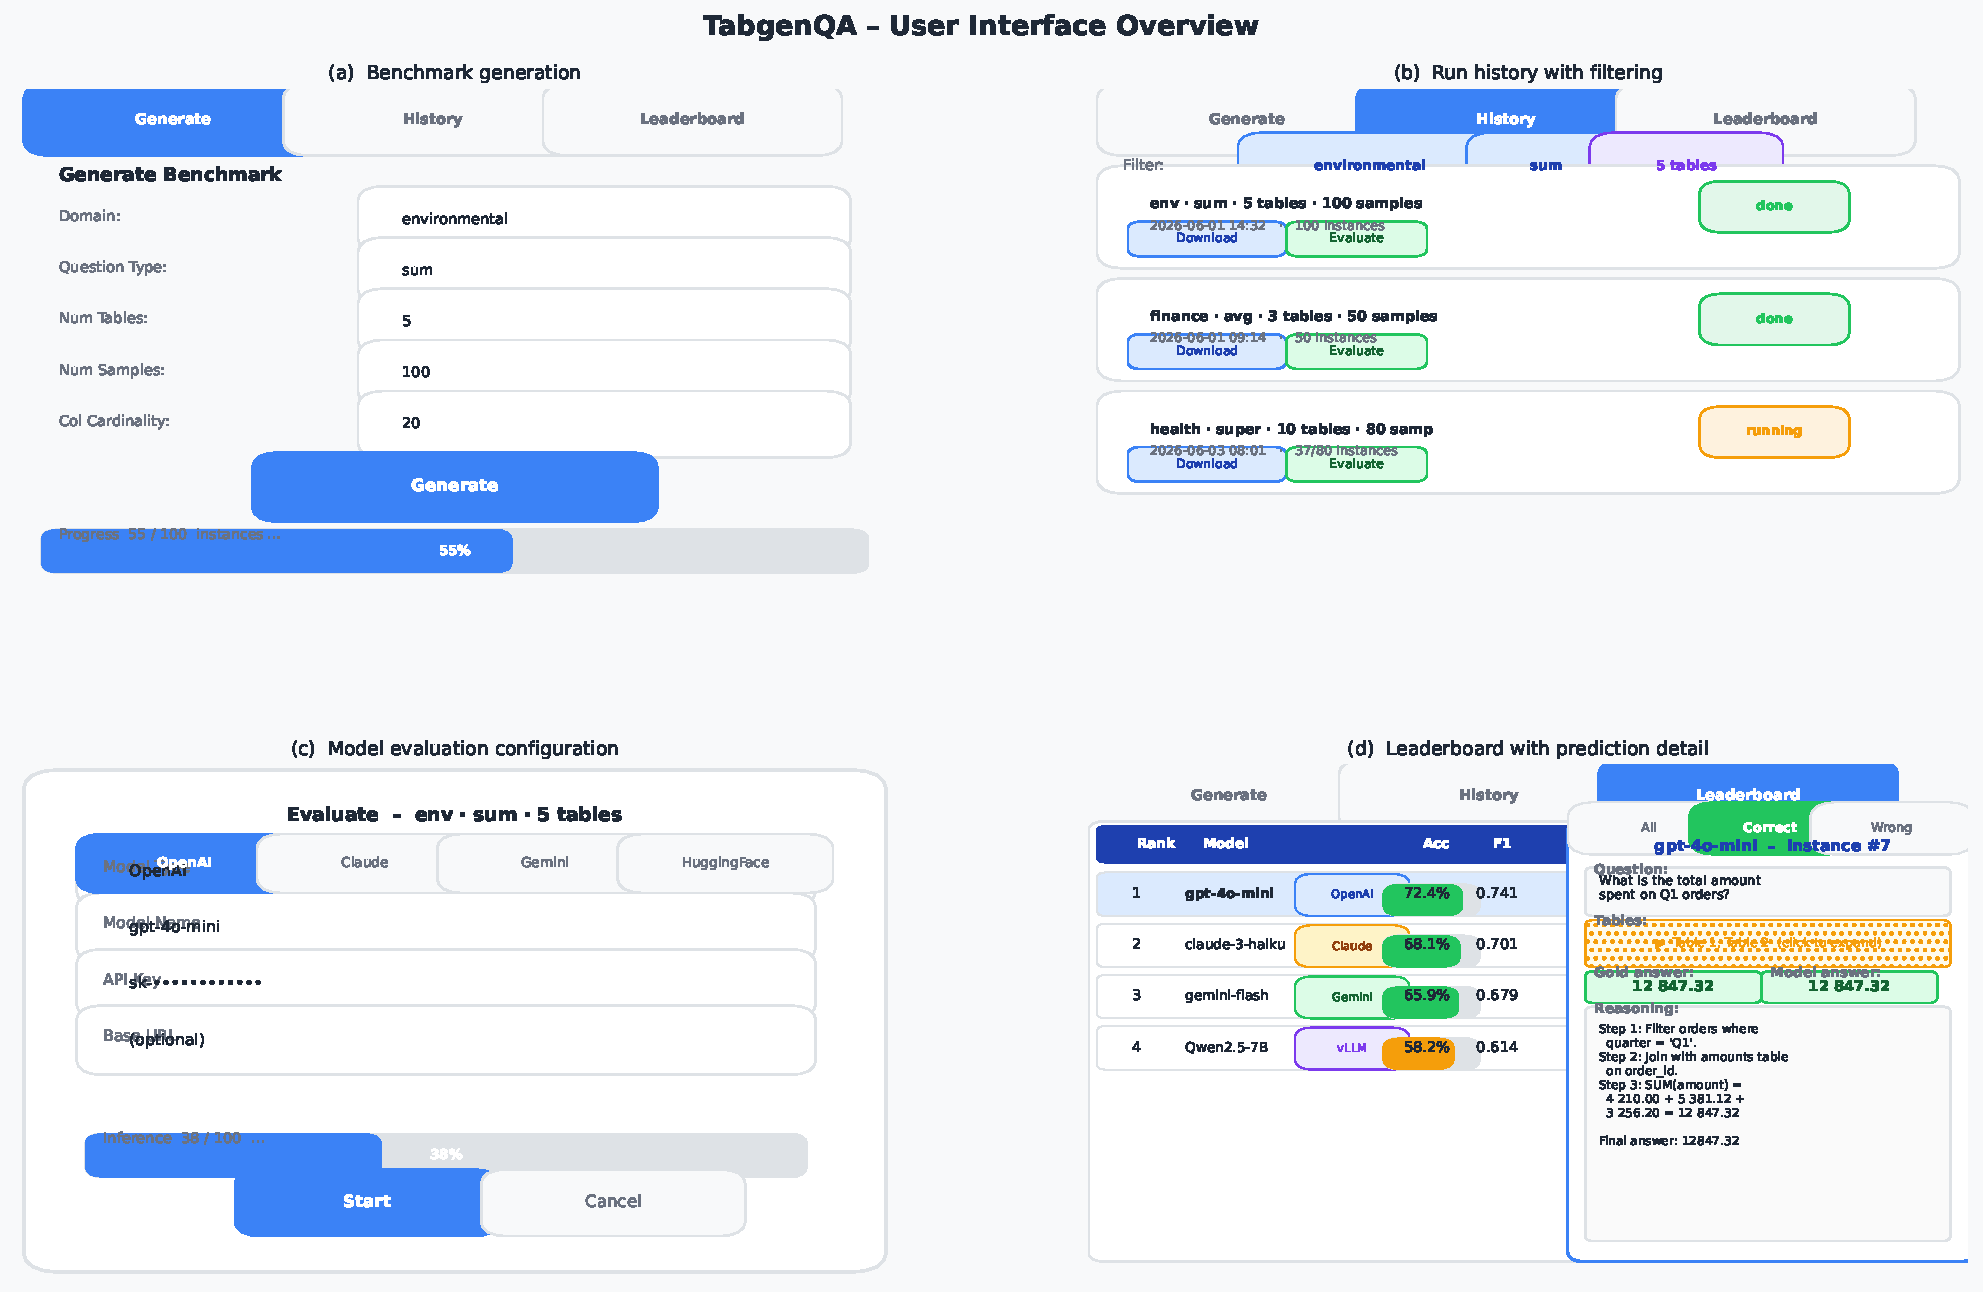
\includegraphics[width=\linewidth]{figures/ui_overview}
  \caption{TabgenQA user interface.
    (a)~Benchmark generation form with SSE progress feedback.
    (b)~History tab with filter controls and per-run actions.
    (c)~Evaluation modal with model and API configuration.
    (d)~Leaderboard with per-instance prediction detail panel.}
  \label{fig:ui}
\end{figure}
